
%(BEGIN_QUESTION)
% Copyright 2011, Tony R. Kuphaldt, released under the Creative Commons Attribution License (v 1.0)
% This means you may do almost anything with this work of mine, so long as you give me proper credit

Create a computer spreadsheet to calculate the required transmitter signal power given frequency, path distance, antenna gains, cable losses, and receiver sensitivity (the minimum signal power required at the receiver input).  A sample layout is presented here, where yellow shading represents values to enter, and blue shading represents values calculated by the spreadsheet:

$$\includegraphics[width=15.5cm]{i00331x01.eps}$$

Then, use your spreadsheet to calculate the minimum transmitter power for a radio system with the following parameters:

\begin{itemize}
\item{} Frequency = 900 MHz
\item{} Path distance = 720 meters
\item{} Receiver sensitivity = $-109$ dBm
\item{} Transmitter cable = $-0.25$ dB per foot ; 12 feet long
\item{} Transmitter lightning arrestor = $-0.2$ dB insertion loss
\item{} Transmitter antenna = 6 dB gain
\item{} Receiver lightning arrestor = $-0.2$ dB insertion loss
\item{} Receiver cable = $-0.25$ dB per foot ; 16 feet long
\item{} Receiver antenna = 13 dB gain
\end{itemize}

\vskip 20pt \vbox{\hrule \hbox{\strut \vrule{} {\bf Suggestions for Socratic discussion} \vrule} \hrule}

\begin{itemize}
\item{} Explain why it is important to have a practical example calculation ready to {\it test} your spreadsheet program.
\item{} How could you alter your spreadsheet to calculate a {\it fade margin} to account for losses due to fade?
\end{itemize}

\underbar{file i00331}
%(END_QUESTION)





%(BEGIN_ANSWER)

The minimum transmitter power required in this application is $-31.92$ dBm which is equal to 0.643 microwatts.

%(END_ANSWER)





%(BEGIN_NOTES)

$$\lambda = {2.9979 \times 10^8 \over 900 \times 10^6} = 0.3331 \hbox{ m}$$

$$L_p = -20 \log \left(4 \pi 720 \over 0.3331\right) = -88.679 \hbox{ dB}$$

\noindent
Where,

$L_p$ = Path loss, a negative dB value

$D$ = Distance between transmitting and receiving antennas

$\lambda$ = Wavelength of transmitted RF field, in same physical unit as $D$

\vskip 10pt

% No blank lines allowed between lines of an \halign structure!
% I use comments (%) instead, so that TeX doesn't choke.

$$\vbox{\offinterlineskip
\halign{\strut
\vrule \quad\hfil # \ \hfil & 
\vrule \quad\hfil # \ \hfil \vrule \cr
\noalign{\hrule}
%
% First row
{\bf Gain or Loss} & {\bf Decibel value} \cr
%
\noalign{\hrule}
%
% Another row
Transmitter cable loss & $-3$ dB \cr
%
\noalign{\hrule}
%
% Another row
Transmitter arrestor loss & $-0.2$ dB \cr
%
\noalign{\hrule}
%
% Another row
Transmitter antenna gain & +6 dBi \cr
%
\noalign{\hrule}
%
% Another row
Path loss & $-88.679$ dB \cr
%
\noalign{\hrule}
%
% Another row
Fade margin & 0 dB \cr
%
\noalign{\hrule}
%
% Another row
Receiver antenna gain & +13 dBi \cr
%
\noalign{\hrule}
%
% Another row
Receiver arrestor loss & $-0.2$ dB \cr
%
\noalign{\hrule}
%
% Another row
Receiver cable loss & $-4$ dB \cr
%
\noalign{\hrule}
%
% Another row
$G_{total} + L_{total}$ & {\bf $-$77.07935 dB} \cr
%
\noalign{\hrule}
} % End of \halign 
}$$ % End of \vbox


\vskip 10pt

$$P_{tx} = P_{rx} - (G_{total} + L_{total})$$

$$P_{tx} = -109 \hbox{ dBm} - ( -77.07935 \hbox{ dB})$$

$$P_{tx} = -31.92 \hbox{ dBm} = 0.00064259 \hbox{ mW} = 0.64259 \> \mu\hbox{W}$$

%INDEX% Computer spreadsheet exercise: RF link budget calculator
%INDEX% Electronics review, RF link budget calculation

%(END_NOTES)


